\documentclass[times,11pt]{article}
%\usepackage[top=1cm, bottom=1cm, left=2.5cm, right=2.5cm]{geometry}

\usepackage{amsmath,amsfonts,amsthm}
\usepackage[pdftex]{graphicx}
\usepackage{float}
\usepackage{url}
\usepackage{natbib}

\numberwithin{equation}{section}		% Equationnumbering: section.eq#
\numberwithin{figure}{section}			% Figurenumbering: section.fig#
\numberwithin{table}{section}				% Tablenumbering: section.tab#

\graphicspath{ {./images/} }

%%% MACROS %%%

\newcommand{\ltwonorm}[1]{\left|\left|{#1}\right|\right|}

%%%%%%%%%%%

\begin{document}

\title{Cache-Friendly Shuffles for Asynchronous Stochastic Optimization}

\maketitle
\section{Introduction}

In modern machine learning, many problems can be cast as instances of optimization, where the goal is to minimize some loss
function encoding the system's errors on training data. The ubiquity of such problems has led to substantial interest in making large-scale
optimization as efficient as possible, and a substantial portion of this work has focused on developing asynchronous algorithms that can under certain regimes
achieve near-ideal speedups in shared-memory systems.

% Introduce Hogwild.
So called {\it stochastic} optimization algorithms have found particular success in this regard. These algorithms, of which stochastic gradient descent (SGD) is the simplest example, operate
on problems whose loss functions decompose as a sum over datapoints:
\begin{align*}
F\left(x\right) & = \sum_{i = 1}^{n} f_{i}\left(x\right) .
\end{align*}
SGD then proceeds by iteratively pulling out the loss function $f_{i}$ for a specific datapoint, updating the model $x$ based on that data point alone, and then moving on to the next one.
SGD and its close cousins have the advantage of being very simply parallelizable. Indeed, the Hogwild algorithm~\citep{} simply spawns $p$ threads to perform the single data point updates in parallel,
allowing them to all update the model without any synchronization whatsoever. Perhaps surprisingly, this lock-free asynchronous approach works well for many problems, and since it avoids communication entirely,
we might hope to achieve ideal speedups and thereby solve even the largest optimization problems facing machine learning practitioners.

% Theory.

% Explain systems issues at high level.
Unfortunately, the simple story fails for a number of reasons, many of them systems-related. As the number of threads becomes large, the architecture of the machine
imposes limitations and tradeoffs that must be taken into account. For instance, many machines with sufficiently many cores to support parallelism beyond approximately $16$
threads organize their cores in a non-uniform memory access (NUMA) architecture, meaning that implementations of Hogwild must either cope with potentially long cross-NUMA node
accesses to the memory storing the model or alter the algorithm so that cores on a given node usually only access memory on that node.

Even on a single node, issues of memory access create pitfalls that must be taken into account. In particular, cache locality and false sharing hamper performance,
and prevent the attainment of ideal speedups with multiple threads.

% Discuss related work (e.g. DimmWitted, Buckwild, Jellyfish)

% Introduce our approach

% Give overview of the report

\subsection{Overview of the report}

\section{A Simplified Memory Model Analysis}

\section{Least Squares}

\section{Word Embeddings}


\subsection{Problem statement}
In the word embeddings problem, given context counts $X_{w,w'}$ we want to find word vectors
$v_{w} \in \mathbb{R}^{k}$ that minimizes the loss:
\begin{align*}
\min_{v,C}\sum_{w,w'}X_{w,w'} \left(\log(X_{w,w'}) - \ltwonorm{v_w+v_{w'}}^2 - C\right)^2
\end{align*}

\subsection{Experimental evaluation}
\subsubsection{Methodology}

We ran our experiments on the Edison compute nodes which feature two
twelve core 2.4 GHz processors. However, we used only up to twelve
cores/threads to avoid effects of NUMA. Word vectors were length 100
double arrays.
\\\\
We used the first $10^9$ bytes of English Wikipedia from
http://mattmahoney.net/dc/textdata as corpus data. After running the text
preprocessing script supplied by the link, we computed co-occurrence
counts of pairs of distinct words to create the parameter dependence graph.
This graph was then fed into gpmetis, computing a min-k-cut partitioning to
create a cache-friendly ordering of the datapoints. k was set such that each
block of k datapoints would reference just enough word vectors to fit into the
L1-cache.
\\\\
Hogwild was then run on the permuted co-occurrence graph generated by gpmetis,
maintaining the same ordering throughout execution. Although we experimented with
both data sharding and no-data sharding, only results from data sharding are presented.
To test hogwild without a cache-friendly shuffle, we randomly shuffled the datapoints before execution.
\\\\
We also ran the experiments on subsets of the corpus, repeating the
procedure on the first $\%10$, $\%25$, $\%50$ and $\%75$ of the corpus data.
In the full corpus data, there were $~200,000$ word vectors, and $~30,000,000$
datapoints.

\subsubsection{Results}
We achieve between $\%40-\%50$ speedup over regular hogwild (non-cache-friendly hogwild),
measuring runtime to a fixed number of epochs.
\begin{figure}[H]
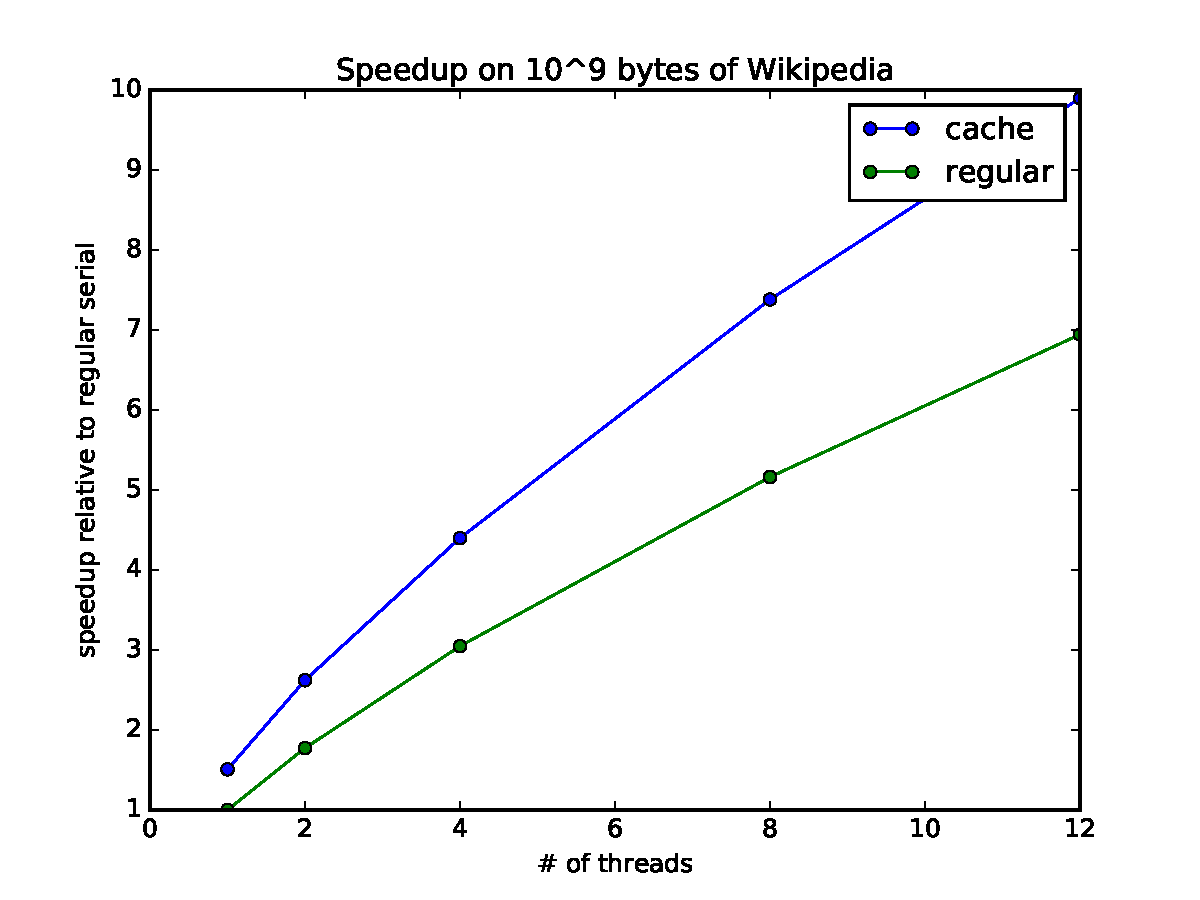
\includegraphics[width=11cm,height=11cm,keepaspectratio]{w2v_speedup_plot.pdf}
\end{figure}
Furthermore, the speedup is maintained on different subsets and sizes of the data.
\begin{figure}[H]
\begin{center}
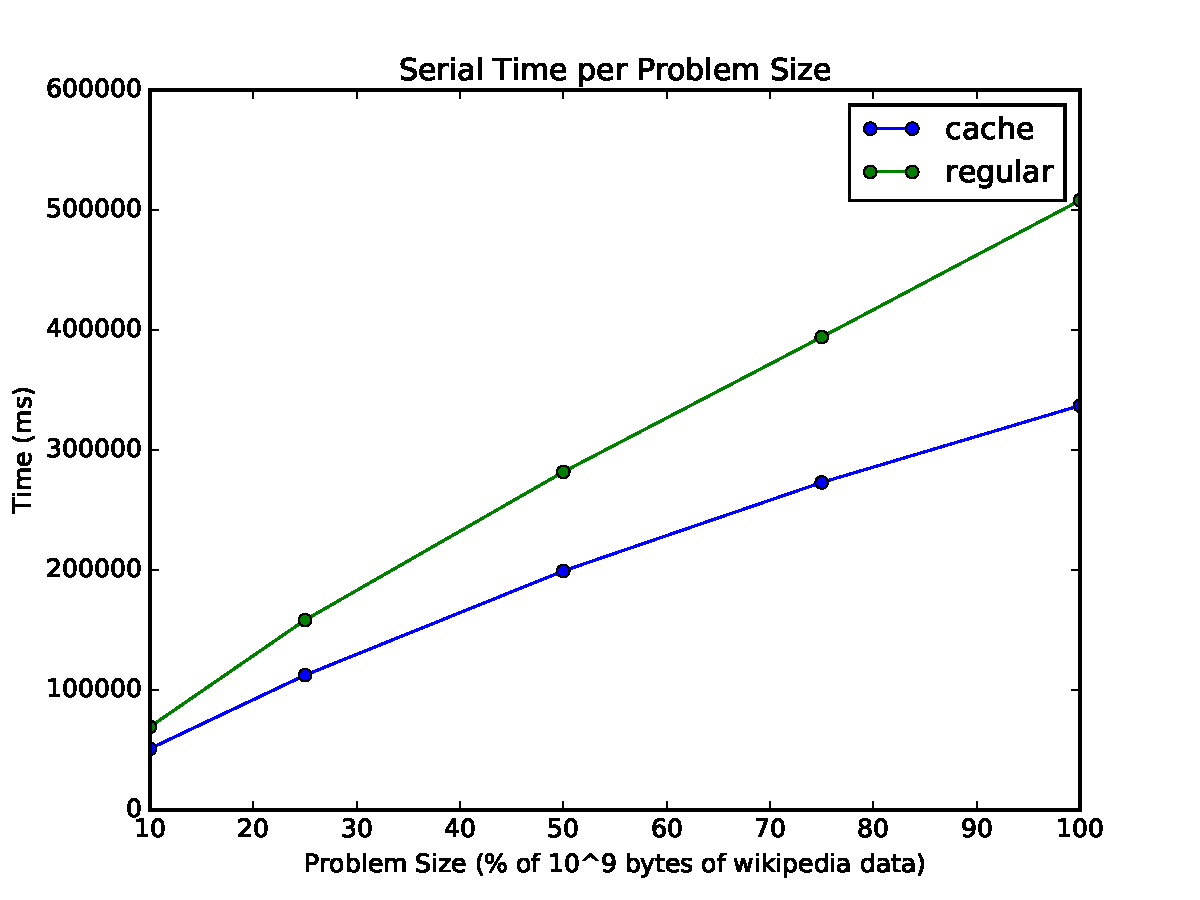
\includegraphics[width=11cm,height=11cm,keepaspectratio]{w2v_problem_size_time_plot.pdf}
\end{center}
\end{figure}
Additionally, convergence of loss is not adversely affected.
\begin{figure}[H]
\begin{center}
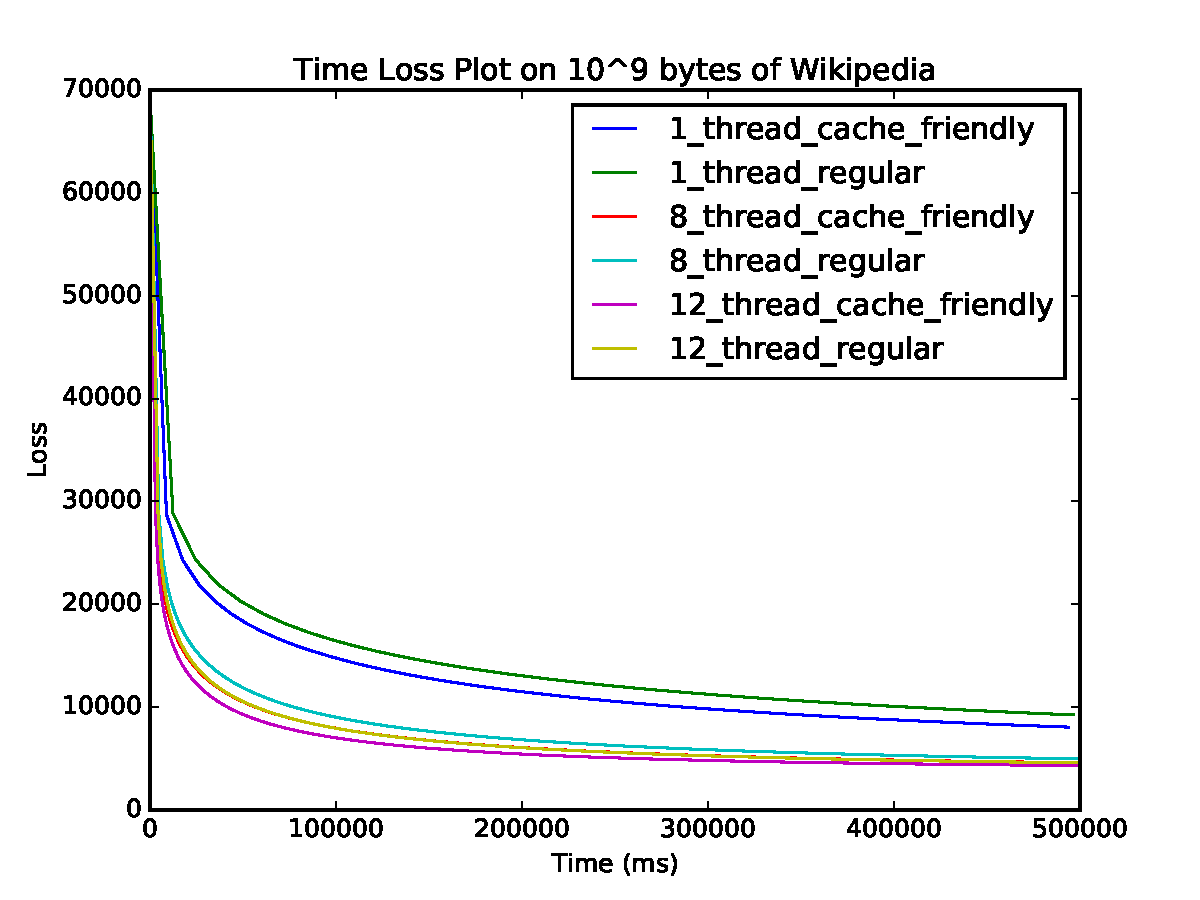
\includegraphics[width=11cm,height=11cm,keepaspectratio]{w2v_time_loss_plot.pdf}
\end{center}
\end{figure}

\subsection{Discussion}

A $\%40-\%50$ runtime gain over regular hogwild is a result of keeping
at least one length 100 double array in the L1-cache between
stochastic gradient calls. In a non-cache-friendly permutation, each
of the two vectors visited by a datapoint is typically not in the
cache, incurring two vectors worth of cache misses per
datapoint. After running min-k-cut on the parameter dependence graph,
we found that each block of k datapoints references around k distinct
vectors. Thus, in a cache-friendly permutation, one of the vectors
referenced by a datapoint is already in the L1-cache from the previous
stochastic gradient call. So a cache-friendly permutation incurs only
one vectors worth of cache misses per datapoint, naturally leading to
a $\%40-\%50$ reduction in runtime.
\newpage
\section{Conclusion}
By ordering datapoints so that model parameters are accessed in a cache friendly manner, we achieve substantial runtime reductions.

% Conclusion for LS

% Conclusion for W2V
For word embeddings, we achieve a $\%40-\%50$ runtime gain over regular hogwild by ordering the datapoints via min-k-cut.

% Overall Conclusion
From these results we believe that using a cache friendly shuffling of datapoints is a promising approach to reducing the runtime of stochastic optimization methods.

\newpage
\section{Future}
The runtime gains achieved by using a cache-friendly shuffle is highly
contingent on the structure of the parameter depedence graph and on
the method used to permute the datapoints. Thus, one possible
direction to explore is the behavior of cache-friendly shuffles on
different graph structures and problem types. We may find that graph
properties such as sparsity, etc, have a nontrivial effect on the
efficacy of cache-friendly shuffles.
\\\\
Different shuffling methods and
heuristics for shuffling may be another topic of exploration. In
particular, the tradeoff between computational efficiency and shuffle
quality may be explored. Investigating different greedy methods and heuristics for
greedy shuffles may reveal computationally efficient methods for
generating a quality cache shuffe. On the other hand, it may also be
interesting to see how effective optimal shuffles are, perhaps by
generating them through some sort of integer linear programming
routine.
\\\\
Finally, a shuffling that takes advantage of all levels of cache may yield further runtime gains.
Thus, a cache-oblivious method shuffling method may be yet another area for exploration.

\end{document}
